% WACV 2027 submission — Post-Training Top-k Checkpoint Averaging
%
% Toggle review / camera-ready on the \usepackage line below.
% Remember to set \wacvPaperID once CMT assigns it.

\documentclass[10pt,twocolumn,letterpaper]{article}

%%%%%%%%% PAPER TYPE  - PLEASE UPDATE FOR FINAL VERSION
\usepackage[review,algorithms]{wacv}      % REVIEW version, algorithms track
% \usepackage[review,applications]{wacv}  % REVIEW version, applications track
% \usepackage{wacv}                       % CAMERA-READY version

%
% --- inline annotations
%
\newcommand{\red}[1]{{\color{red}#1}}
\newcommand{\todo}[1]{{\color{red}#1}}
\newcommand{\TODO}[1]{\textbf{\color{red}[TODO: #1]}}
% --- disable by uncommenting
% \renewcommand{\TODO}[1]{}
% \renewcommand{\todo}[1]{#1}

\usepackage{amsmath}
\usepackage{amssymb}
\usepackage{booktabs}
\usepackage{multirow}
\usepackage{makecell}
\usepackage{array}
\usepackage{graphicx}
\usepackage{xcolor}
\usepackage{colortbl}
\usepackage{algorithm}
\usepackage{algpseudocode}
\usepackage{subcaption}

% ── Results-table helpers ────────────────────────────────────────────────
% \ms{mean}{std} — plain cell;  \best{mean}{std} — highlighted best in block
\newcommand{\ms}[2]{$#1${\scriptsize$\,\pm#2$}}
\newcommand{\best}[2]{\cellcolor{black!8}$\mathbf{#1}${\scriptsize$\,\pm#2$}}


\definecolor{wacvblue}{rgb}{0.21,0.49,0.74}
\usepackage[pagebackref,breaklinks,colorlinks,allcolors=wacvblue]{hyperref}

%%%%%%%%% PAPER ID  - PLEASE UPDATE
\def\wacvPaperID{*****} % *** Enter the WACV Paper ID here
\def\confName{WACV}
\def\confYear{2027}

%%%%%%%%% TITLE
\title{Criterion-Guided Top-$k$ Checkpoint Averaging:\\
A Post-Training Model-Selection Rule for Classification, Detection and Segmentation}

%%%%%%%%% AUTHORS - anonymous for review; fill in for camera-ready
\author{Anonymous \confName~submission\\
Paper ID \wacvPaperID}

\begin{document}
\maketitle

\begin{abstract}
Standard training pipelines finalize a model by keeping the single checkpoint
that scores best on a validation split. That decision is winner-takes-all, and
late-epoch validation metrics fluctuate enough that the winner is partly
determined by noise. We propose a post-training model-selection rule that
replaces it: rank the epoch checkpoints of a \emph{completed} run by the same
validation criterion already used to pick the best one, keep the top $k$, and
uniformly average their parameters. No optimizer, schedule, or training budget
is changed, no secondary optimization is introduced, and inference cost is that
of a single model. All it needs is a way to order the checkpoints, so it transfers across tasks
unchanged: we rank by validation loss for classification and by validation
fitness for detection and segmentation.
We evaluate 34 model--dataset configurations---six classification
architectures on five datasets, two detectors on PASCAL VOC, and two
segmentation models on Carparts---with five seeds each, every variant sharing
its baseline's training trajectory so that only the selection rule differs. At
the common setting $k{=}5$, the primary metric improves in all 34
configurations. Equally weighted over the 30 classification configurations,
accuracy rises from 81.73\% to 83.76\% and macro-F1 from 81.65\% to 83.86\%,
while detection and segmentation fitness gain 5.8--6.9\% relative. Across-seed
standard deviation falls by roughly a fifth. Finally, we show that the selected
checkpoints are typically neither contiguous nor concentrated at the end of
training, which is precisely what separates the rule from last-$k$ temporal
averaging.
\end{abstract}

\section{Introduction}
\label{sec:intro}

\begin{figure}[t]
  \centering
  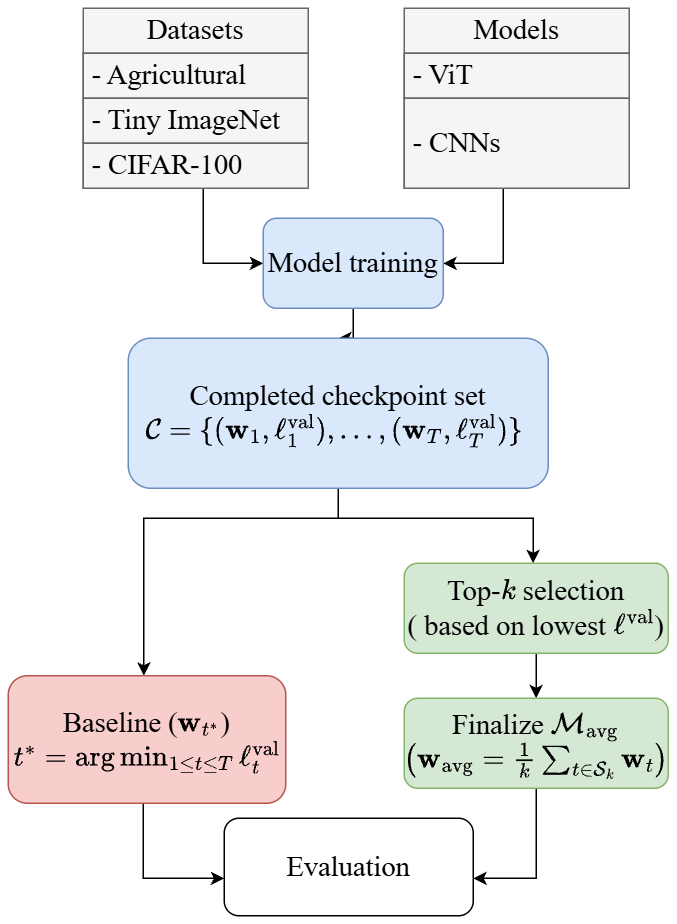
\includegraphics[width=\linewidth]{Pipeline.png}
  \caption{The rule operates only at the model-selection stage. Training runs
    unmodified and emits a checkpoint set; the baseline keeps the single
    best-scoring state, while we keep the top $k$ by the same criterion, average
    their trainable parameters, and recompute Batch-Normalization statistics
  before the final evaluation.}
  \label{fig:pipeline}
\end{figure}

Nearly every supervised vision pipeline ends with the same step. Training
produces a sequence of epoch checkpoints, each is scored on a held-out
validation split, and the single best-scoring state is kept as the final model
\cite{bishop2006pattern,prechelt2002early}. The step is so routine that it is
rarely reported, let alone questioned. Yet it is a winner-takes-all decision
taken on a noisy statistic: late-epoch validation metrics fluctuate under
mini-batch sampling, stochastic optimization, and the finite size of the
validation split \cite{prechelt2002early,izmailov2019averagingweightsleadswider,garipov2018losssurfacesmodeconnectivity},
and checkpoints with near-identical training loss can generalize
measurably differently \cite{keskar2017largebatchtrainingdeeplearning}. The gap
between the best and second-best epoch is often well inside that noise, so
which one wins is partly an accident of the run.

Aggregating several states rather than committing to one is the natural
response. Prediction-time ensembling does this but multiplies inference cost by
the ensemble size \cite{dietterich2000ensemble}. Weight averaging avoids that:
averaging parameters instead of outputs yields a single model at single-model
cost. Iterate averaging is classical \cite{polyak1992acceleration}, and SWA
\cite{izmailov2019averagingweightsleadswider} showed that averaging states
sampled along a trajectory finds flatter, better-generalizing optima. The catch
is that these methods intervene in training: SWA prescribes an additional SGD
phase with a prescribed learning-rate schedule, LAWA \cite{kaddour2022stop}
averages inside the training loop on a recency window, and TWA
\cite{li2022trainable} adds a secondary optimization for the coefficients. Each
asks the practitioner to modify a pipeline that already works.

\paragraph{This paper.}
We ask what can be gained by changing nothing except the final selection step.
Our rule operates strictly after a standard run has terminated. It reuses the
validation criterion the pipeline already computes to rank checkpoints, takes
the top $k$, and averages their trainable parameters uniformly
(\cref{fig:pipeline}). Batch-Normalization statistics are recomputed with a
single gradient-free pass, as in SWA. Nothing else changes: not the optimizer,
the schedule, the early-stopping rule, nor the epoch budget. The result is one
set of weights with the inference cost of one model.

The rule's only interface to the task is a scalar criterion per checkpoint,
which is what makes it portable. Classification pipelines rank by validation
loss; detection and segmentation pipelines already rank by a validation
\emph{fitness} score. We plug in whichever the pipeline uses and the procedure
is otherwise identical, which lets us evaluate the same rule on three tasks
without task-specific tuning.

\paragraph{Why top-$k$ by criterion and not the last $k$.}
Averaging the final $k$ checkpoints is established practice, notably in machine
translation \cite{vaswani2017attention,junczys2016neural}. It selects by
position in the training sequence, which is a proxy for quality that holds only
if late training is stable. Our rule selects by measured validation quality
instead, so the chosen set may skip epochs and may reach back well before the
end of the run. \Cref{sec:selection} shows this is not a hypothetical
difference: on CIFAR-100, only 5 of 30 runs yield a contiguous set, and just
11.3\% of selected checkpoints fall in the final five epochs, so a last-$k$
window would average a largely disjoint set of weights.

\paragraph{Contributions.}
\begin{enumerate}
\itemsep0em
\item A post-training, criterion-guided top-$k$ averaging rule that requires no
change to the training pipeline, no secondary optimization, and no additional
inference cost, and that is specified independently of the task
(\cref{sec:method}).
\item An evaluation spanning three tasks and 34 model--dataset configurations
under a matched-trajectory protocol in which the baseline and every $k$ are
derived from the same completed run and the same seed, so that differences are
attributable to the selection rule alone (\cref{sec:results}). At $k{=}5$ the
primary metric improves in all 34 configurations.
\item An analysis of \emph{which} checkpoints the criterion selects, which
establishes empirically that criterion-ranked and temporal-window selection
pick different sets, and quantifies the storage this costs
(\cref{sec:selection}).
\end{enumerate}

\section{Related Work}
\label{sec:related}

\paragraph{Training-time weight averaging.}
Averaging iterates reduces variance and improves asymptotic convergence
\cite{polyak1992acceleration}. Exponential Moving Average applies the idea
online, maintaining a smoothed parameter copy throughout training
\cite{tarvainen2018meanteachersbetterrole}; because the average is taken over
the whole history, it retains influence from early, weak states. SWA
\cite{izmailov2019averagingweightsleadswider} averages states sampled along an
SGD trajectory under a cyclical or constant learning-rate schedule, starting
from a conventionally trained model and continuing optimization. Its algorithm
therefore prescribes learning-rate bounds, a cycle length, and an iteration
budget. LAWA \cite{kaddour2022stop} keeps a sliding window of the $k$ most recent
checkpoints and periodically replaces the live model with their average during
training; its candidates are chosen by recency, independent of how each
checkpoint scores. TWA \cite{li2022trainable} learns the averaging coefficients
in the subspace spanned by the candidates, improving over SWA at the cost of a
secondary optimization stage.

Our rule differs from all of these in when it acts and in what it needs. It
runs after training has terminated, prescribes no optimizer, schedule, cycle
structure or stopping rule, and performs no secondary optimization. It requires
only that epoch checkpoints and their validation scores exist, which standard
pipelines already produce.

\paragraph{Inference-time ensembling.}
Combining diverse hypotheses improves generalization at inference cost
proportional to ensemble size \cite{dietterich2000ensemble}. Snapshot ensembles
reduce the \emph{training} cost of obtaining diverse members by exploiting
cyclical learning rates within one run \cite{huang2017snapshotensemblestrain1},
but the inference overhead remains. Our setting assumes that overhead is not
available.

\paragraph{Post-training aggregation.}
Temporal-window averaging selects checkpoints by position: the last $k$ epochs,
or checkpoints at fixed intervals. Transformers popularized it
\cite{vaswani2017attention} and neural machine translation adopted it as
convention \cite{junczys2016neural}, on the assumption that recent checkpoints
have reached a stable region and are interchangeable. When late-stage
validation is non-monotonic---through transient optimization noise,
overfitting, or scheduler effects---a fixed window can admit degraded
checkpoints and exclude stronger ones outside it, so the average depends on
where training happened to stop rather than on measured quality.

Model Soups \cite{wortsman2022model} also filter candidates by a validation
criterion before averaging: the greedy variant admits a fine-tuned model only
if it improves validation accuracy. The structural difference is the candidate
pool. Soups average \emph{across independently trained models} from a
hyperparameter sweep, so they presuppose that sweep; our rule averages
\emph{within a single run}, over the epoch checkpoints that run already
produced. The two are complementary rather than competing.

\paragraph{Positioning.}
Prior post-training averaging work is largely confined to one task family, and
the closest temporal alternative---last-$k$---has not been contrasted with
criterion ranking in terms of \emph{which checkpoints are actually selected}.
\Cref{sec:selection} supplies that comparison.

\section{Method}
\label{sec:method}

\subsection{Setting}

A standard run produces a checkpoint set
$\mathcal{C}=\{(\mathbf{w}_t,\, c_t)\}_{t=1}^{T}$, where $\mathbf{w}_t$ are the
parameters after epoch $t$ and $c_t$ is the scalar validation criterion the
pipeline already records at that epoch, on a split disjoint from the final
evaluation set. Pipelines differ in whether that criterion is minimized (a
loss) or maximized (a performance score), so we first remove the distinction.
Let $\delta=-1$ if the pipeline minimizes $c_t$ and $\delta=+1$ if it maximizes
it, and define the \emph{selection score}
\begin{equation}
  s_t \;=\; \delta \cdot c_t ,
  \label{eq:score}
\end{equation}
which is oriented so that larger is always better. Everything below is written
in terms of $s_t$ and is therefore identical for both kinds of pipeline.
Conventional selection keeps the single best state,
\begin{equation}
  t^{*}=\operatorname*{arg\,max}_{1\le t\le T} s_t ,
  \qquad
  \mathbf{w}_{\text{base}}=\mathbf{w}_{t^{*}} .
  \label{eq:baseline}
\end{equation}

\subsection{Criterion-Guided Top-$k$ Averaging}

Instead of the single maximizer we take the $k$ best-scoring epochs,
\begin{equation}
  \mathcal{S}_k=\operatorname*{arg\,max}_{\substack{\mathcal{S}\subseteq\{1,\dots,T\}\\ |\mathcal{S}|=k}}\ \sum_{t\in\mathcal{S}} s_t ,
  \label{eq:topk}
\end{equation}
that is, the indices of the $k$ largest $s_t$, and average their trainable
parameters element-wise:
\begin{equation}
  \mathbf{w}_{\text{avg}}=\frac{1}{|\mathcal{S}_k|}\sum_{t\in\mathcal{S}_k}\mathbf{w}_t .
  \label{eq:avg}
\end{equation}
Ties are broken in favour of later epochs, matching the convention by which
standard pipelines overwrite their best checkpoint on an equal score. Because
\cref{eq:topk} depends on $s_t$ only through its ordering, any strictly
monotone reparameterization of the criterion leaves $\mathcal{S}_k$ unchanged;
$\delta$ in \cref{eq:score} is the only task-dependent quantity in the method.

Two structural properties follow. First, $\mathcal{S}_1=\{t^{*}\}$, so
\cref{eq:baseline} is the $k{=}1$ case of \cref{eq:topk}: the baseline is
nested inside the method rather than being a separate procedure. Second,
$\mathcal{S}_{k-1}\subset\mathcal{S}_k$, so increasing $k$ only admits one
further checkpoint and never displaces an existing one.

\paragraph{Normalization statistics.}
Averaging is applied to trainable parameters only. Batch-Normalization
\cite{ioffe2015batch} running statistics are population estimates tied to the
particular weights that produced them, so those inherited from any single
member need not match $\mathbf{w}_{\text{avg}}$. Following SWA
\cite{izmailov2019averagingweightsleadswider} we reset them and recompute them
with forward passes over training data in training mode, without gradients or
optimizer updates. This is the method's only compute overhead and it is paid
once.

\subsection{Instantiating the Criterion}

The rule touches the task only through the pair $(c_t,\delta)$, which is why it
transfers without modification. We use whichever criterion the pipeline already
computes to select its own best checkpoint, so the method never introduces a
quantity the pipeline was not already tracking:

For \textbf{classification}, $c_t$ is the validation cross-entropy loss and
$\delta={-}1$, giving $s_t=-\ell^{\text{val}}_t$. For \textbf{detection and
segmentation}, $c_t$ is the validation fitness $\varphi_t$ and $\delta={+}1$,
giving $s_t=\varphi_t$; we read $\varphi_t$ straight from the Ultralytics
trainer \cite{jocher2023ultralytics}, which defines it as
$0.1\,\mathrm{mAP}_{50}+0.9\,\mathrm{mAP}_{50:95}$ for detection and as the sum
of that quantity over the box and mask components for segmentation. In both
cases it is the same scalar the pipeline uses for its own best checkpoint and
for early stopping, so baseline and rule are ranked by an identical signal.

No part of \cref{eq:topk,eq:avg} is task-specific, and we tune nothing per task
beyond setting $\delta$. The rule consequently inherits whatever biases the
pipeline's criterion already has: if the criterion is a poor proxy for test
performance, ranking by it will not repair that.

\subsection{Procedure and Cost}

\begin{algorithm}[t]
\caption{Criterion-guided top-$k$ checkpoint averaging}
\label{alg:topk}
\begin{algorithmic}[1]
\Require completed checkpoint set $\{(\mathbf{w}_t,c_t)\}_{t=1}^{T}$;
aggregation size $k\le T$; criterion direction
$\delta\in\{-1,+1\}$ ($-1$ if $c_t$ is a loss, $+1$ if it is a
score); training data $\mathcal{D}_{\text{train}}$
\Ensure final model $\mathcal{M}_{\text{avg}}$
\Statex \textbf{Rank} --- orient the criterion, then select
\For{$t=1,\dots,T$}
  \State $s_t \gets \delta\cdot c_t$ \Comment{larger is better}
\EndFor
\State $\mathcal{S}_k \gets$ indices of the $k$ largest $s_t$,
ordering ties by larger $t$
\Statex \textbf{Average} --- trainable parameters only
\State $\mathbf{w}_{\text{avg}} \gets \frac{1}{k}\sum_{t\in\mathcal{S}_k}\mathbf{w}_t$
\State load $\mathbf{w}_{\text{avg}}$ into $\mathcal{M}_{\text{avg}}$
\Statex \textbf{Recalibrate} --- only if normalization buffers exist
\If{$\mathcal{M}_{\text{avg}}$ has BatchNorm layers}
  \State reset their running mean and variance
  \State \textbf{for} a fixed number of batches from
  $\mathcal{D}_{\text{train}}$ \textbf{do} forward pass in training
  mode, no gradients, no optimizer step
\EndIf
\State \Return $\mathcal{M}_{\text{avg}}$
\end{algorithmic}
\end{algorithm}

\Cref{alg:topk} summarizes the procedure; setting $k{=}1$ recovers the baseline
line for line, which is what makes the two arms comparable. Training cost is
unchanged by construction, post-training cost is $k$ tensor additions plus one
recalibration pass, and inference cost is that of a single model. Storage is
the only real cost and it is bounded: because \cref{eq:topk} depends only on
the ordering of $s_t$, a running set of the $k$ best checkpoints seen so far
yields the same $\mathcal{S}_k$ as ranking the full set offline, so $k{+}1$
states suffice at any moment. Our detection and segmentation runs implement
exactly this, pruning a new checkpoint immediately if it falls outside the
current top $k$; the classification runs retain all epochs and we report the
counts in \cref{sec:selection}.

\paragraph{Implementation details.}
Two choices keep the comparison clean. The Ultralytics trainer validates
through an exponential moving average of the weights by default; we disable
that smoothing so the recorded fitness, the early-stopping signal and the
stored weights all refer to the same raw parameters, since otherwise
checkpoints would be ranked by a quantity computed from weights other than
those being averaged. We also take the baseline from the top-ranked entry of
the same table our rule ranks rather than from the framework's exported best
checkpoint, which is serialized at half precision: comparing it against a
full-precision average would confound the selection rule with a precision
change.

\section{Experimental Setup}
\label{sec:setup}

\subsection{Tasks, Datasets and Protocols}

We evaluate on three tasks. \Cref{tab:datasets} lists the datasets and the
split used at each stage. Throughout, the \emph{selection} split is the one the
criterion $c_t$ is computed on, and it is always disjoint from the split used
for the reported numbers.

\begin{table*}[t]
  \centering
  \small
  \setlength{\tabcolsep}{5pt}
  \caption{Datasets and evaluation protocol. ``Selection'' is the split the
    ranking criterion $c_t$ is computed on; it is disjoint from ``Final
    evaluation'' in every case. Tiny ImageNet publishes no labelled test split,
    so its official validation split is the held-out evaluation set and its
    numbers are reported as validation metrics
    \cite{abai2019densenet,huynh2022vision}. For PASCAL VOC the original
    Ultralytics configuration aliases \texttt{val} to the VOC2007 test split,
    which would let the criterion see the evaluation data; we therefore hold out
  an independent selection split from the training pool.}
  \label{tab:datasets}
  \resizebox{\textwidth}{!}{%
\begin{tabular}{llccll}
    \toprule
    Task & Dataset & Classes & Available images & Selection & Final evaluation \\
    \midrule
    \multirow{5}{*}{Classification}
      & Tomato Leaf Disease \cite{solapure2024tomato}      & 10  & 1,609  & 15\% of set & 15\% test split \\
      & Burmese Grape Leaf Disease \cite{rahman2025burmese}& 5   & 3,103  & 15\% of set & 15\% test split \\
      & Potato Leaf Disease \cite{Shabrina2023Potato}      & 7   & 3,076  & 15\% of set & 15\% test split \\
      & CIFAR-100 \cite{krizhevsky2009learning}            & 100 & 50,000 train + 10,000 test & 5,000 from train & 10,000 official test \\
      & Tiny ImageNet \cite{le2015tiny}                    & 200 & 100,000 train + 10,000 val & 10,000 from train & 10,000 official val.\ \\
    \midrule
    Detection
      & PASCAL VOC \cite{everingham2010pascal}             & 20  & 16,551 trainval + 4,952 test & 1,655 from trainval & 4,952 VOC2007 test \\
    \midrule
    Segmentation
      & Carparts \cite{ultralytics2024carparts}            & 23  & 3,156 train + 401 val + 276 test & held out from train & 276 test split \\
    \bottomrule
  \end{tabular}}
\end{table*}

\paragraph{Classification.}
Three agricultural datasets---Tomato, Burmese Grape and Potato leaf
disease---provide a domain-specific, small-data regime, and CIFAR-100 and Tiny
ImageNet provide standard general-purpose benchmarks. The agricultural sets use
a stratified 70/15/15 train/selection/test partition. CIFAR-100 keeps its
official test split intact and carves 5,000 selection images out of the
training partition. Tiny ImageNet has no publicly labelled test split, so
following common practice on this benchmark
\cite{abai2019densenet,huynh2022vision} its official validation split serves as
the held-out evaluation set; every Tiny ImageNet number we report is therefore
labelled a validation metric, and its selection split is a separate 10,000
images stratified out of the training partition.

\paragraph{Detection.}
PASCAL VOC \cite{everingham2010pascal} in the Ultralytics configuration trains
on the union of the VOC2007 and VOC2012 \texttt{trainval} sets (16,551 images,
20 classes) and evaluates on the VOC2007 test set (4,952 images). That
configuration aliases the \texttt{val} split to the test split, which would
make the selection criterion a function of the evaluation data. We therefore
hold out 10\% of the training pool as an independent selection split and leave
the VOC2007 test set untouched for reporting.

\paragraph{Segmentation.}
Carparts \cite{ultralytics2024carparts} is an instance-segmentation dataset of
vehicle parts with 23 classes and a 3,156/401/276 train/val/test split. As
above, the selection split is held out from the training pool and the test
split is used only for reporting.

\subsection{Models}

For classification we fine-tune six ImageNet-pretrained backbones end-to-end,
instantiated from \texttt{timm} \cite{rw2019timm}, chosen to span
architectural families: VGG16 \cite{simonyan2015vgg} (plain convolutions),
ResNet101 \cite{he2016deep} (residual), DenseNet121 \cite{huang2017densely}
(dense connectivity), MobileNetV2 \cite{sandler2018mobilenetv2} (depthwise
separable, mobile budget), EfficientNetB0 \cite{tan2019efficientnet} (compound
scaling), and ViT-Base \cite{dosovitskiy2021imageworth16x16words}
(transformer). For detection and segmentation we use YOLOv8s
\cite{jocher2023ultralytics} and YOLO11s \cite{jocher2024yolo11}, covering two
generations of the same family. The six classification backbones across five
datasets give 30 configurations; two detectors on VOC and two segmentation
models on Carparts give four more, for 34 in total.

\subsection{Matched-Trajectory Protocol}

Every configuration is trained independently with five seeds
$\{1,10,42,100,500\}$. For a given seed, the baseline and all $k$ are derived
from the \emph{same} completed run and the same checkpoint set, so they share
architecture, initialization, data order, optimizer, schedule and training
duration, and differ only in the post-training selection rule. Any difference
between them is therefore attributable to that rule and not to training
variance. We report mean $\pm$ standard deviation over the five seeds. All
values of $k$ are reported as a sensitivity analysis; $k$ is never chosen using
the final evaluation split.

\subsection{Training Configuration}

Training pipelines are held fixed between the baseline and every $k$, so the
configuration below affects both arms identically and cannot favour either.
\Cref{tab:configs} records the per-model settings.

\begin{table*}[t]
  \centering \small
  \setlength{\tabcolsep}{5pt}\renewcommand{\arraystretch}{1.08}
  \caption{Per-model training configuration. The pipeline is identical for the baseline and every $k$, so these settings affect both arms equally and cannot favour either. \TODO{fill in}}
  \label{tab:configs}
  \resizebox{\textwidth}{!}{%
  \begin{tabular}{@{}llcccc@{\hspace{2.5em}}llcccc@{}}
    \toprule
    Dataset & Model & Batch & Epochs & LR & Patience & Dataset & Model & Batch & Epochs & LR & Patience \\
    \midrule
    \multirow{6}{*}{Tomato Leaf} & ViT-Base & & & & & \multirow{6}{*}{CIFAR-100} & ViT-Base & & & & \\
     & VGG16 & & & & &  & VGG16 & & & & \\
     & ResNet101 & & & & &  & ResNet101 & & & & \\
     & MobileNetV2 & & & & &  & MobileNetV2 & & & & \\
     & DenseNet121 & & & & &  & DenseNet121 & & & & \\
     & EfficientNetB0 & & & & &  & EfficientNetB0 & & & & \\\cmidrule(r){1-6}\cmidrule(l){7-12}
    \multirow{6}{*}{Burmese Grape} & ViT-Base & & & & & \multirow{6}{*}{Tiny ImageNet} & ViT-Base & & & & \\
     & VGG16 & & & & &  & VGG16 & & & & \\
     & ResNet101 & & & & &  & ResNet101 & & & & \\
     & MobileNetV2 & & & & &  & MobileNetV2 & & & & \\
     & DenseNet121 & & & & &  & DenseNet121 & & & & \\
     & EfficientNetB0 & & & & &  & EfficientNetB0 & & & & \\\cmidrule(r){1-6}\cmidrule(l){7-12}
    \multirow{6}{*}{Potato Leaf} & ViT-Base & & & & & \multirow{2}{*}{PASCAL VOC} & YOLOv8s & & & & \\
     & VGG16 & & & & &  & YOLO11s & & & & \\\cmidrule(l){7-12}
     & ResNet101 & & & & & \multirow{2}{*}{Carparts} & YOLOv8s & & & & \\
     & MobileNetV2 & & & & &  & YOLO11s & & & & \\
     & DenseNet121 & & & & &  &  & & & & \\
     & EfficientNetB0 & & & & &  &  & & & & \\\cmidrule(r){1-6}
    \bottomrule
  \end{tabular}}
\end{table*}

\paragraph{Shared settings.}
\TODO{fill in: optimizer, LR schedule and warmup, weight decay, loss,
input resolution, classifier head, augmentation, BN-recalibration batches.}

\section{Results}
\label{sec:results}

\begin{table*}[t]
  \centering \scriptsize
  \setlength{\tabcolsep}{4pt}\renewcommand{\arraystretch}{1.06}
  \caption{Classification accuracy (\%). Mean $\pm$ std over five seeds; $k{=}1$ is the single-checkpoint baseline and shaded bold marks the best $k$ within each dataset block. $^{\dagger}$Tiny ImageNet entries are validation metrics (\cref{tab:datasets}). At $k{=}5$ accuracy beats the baseline in all 30 configurations.}
  \label{tab:results-acc}
  \begin{tabular}{@{}ll cccccc@{}}
    \toprule
    \textbf{Dataset} & $k$ & \textbf{VGG16} & \makecell{\textbf{Dense}\\\textbf{Net121}} & \makecell{\textbf{Efficient}\\\textbf{NetB0}} & \makecell{\textbf{Mobile}\\\textbf{NetV2}} & \makecell{\textbf{ResNet}\\\textbf{101}} & \makecell{\textbf{ViT}\\\textbf{Base}} \\
    \midrule
    \multirow{5}{*}{CIFAR-100} & 1 & \ms{71.57}{0.41} & \ms{75.39}{0.20} & \ms{76.76}{0.51} & \ms{73.23}{0.41} & \ms{75.84}{1.54} & \ms{87.19}{0.65} \\
     & 2 & \ms{72.10}{0.45} & \ms{78.10}{0.20} & \ms{79.85}{0.31} & \ms{74.24}{0.22} & \ms{78.08}{0.28} & \ms{88.68}{0.28} \\
     & 3 & \ms{72.34}{0.40} & \ms{78.73}{0.12} & \ms{80.51}{0.06} & \ms{74.68}{0.24} & \ms{78.60}{0.36} & \ms{89.12}{0.59} \\
     & 4 & \best{72.48}{0.47} & \ms{78.93}{0.18} & \ms{80.92}{0.22} & \ms{74.92}{0.18} & \best{78.82}{0.48} & \ms{89.39}{0.36} \\
     & 5 & \ms{72.46}{0.43} & \best{79.23}{0.30} & \best{81.15}{0.31} & \best{75.06}{0.15} & \ms{78.80}{0.53} & \best{89.64}{0.28} \\
    \midrule
    \multirow{5}{*}{Tiny ImageNet$^{\dagger}$} & 1 & \ms{67.54}{0.85} & \ms{76.82}{0.61} & \ms{80.32}{0.32} & \ms{72.90}{0.54} & \ms{77.50}{0.60} & \ms{89.68}{0.34} \\
     & 2 & \ms{68.04}{0.46} & \ms{77.74}{0.11} & \ms{80.64}{0.25} & \ms{73.39}{0.38} & \ms{80.41}{0.10} & \ms{90.96}{0.15} \\
     & 3 & \ms{68.12}{0.43} & \ms{77.88}{0.13} & \ms{80.72}{0.26} & \ms{73.40}{0.31} & \ms{80.86}{0.13} & \ms{91.31}{0.10} \\
     & 4 & \best{68.35}{0.38} & \best{78.06}{0.15} & \best{80.81}{0.19} & \ms{73.46}{0.23} & \ms{81.23}{0.14} & \ms{91.43}{0.10} \\
     & 5 & \ms{68.34}{0.35} & \ms{78.04}{0.22} & \ms{80.78}{0.20} & \best{73.53}{0.21} & \best{81.34}{0.32} & \best{91.53}{0.12} \\
    \midrule
    \multirow{5}{*}{Burmese Grape} & 1 & \ms{83.76}{2.04} & \ms{84.62}{1.62} & \ms{82.74}{2.09} & \ms{83.89}{1.54} & \ms{85.38}{0.94} & \ms{86.98}{1.92} \\
     & 2 & \ms{85.30}{1.39} & \ms{84.96}{1.34} & \ms{85.56}{1.27} & \ms{85.94}{2.28} & \ms{85.13}{1.49} & \ms{86.58}{2.18} \\
     & 3 & \ms{85.43}{0.84} & \ms{85.00}{1.50} & \ms{85.77}{0.74} & \ms{86.67}{1.53} & \ms{85.17}{1.61} & \best{87.05}{1.44} \\
     & 4 & \ms{85.77}{0.93} & \ms{84.96}{1.40} & \best{86.54}{1.05} & \best{87.19}{1.54} & \best{85.68}{1.41} & \ms{86.79}{1.47} \\
     & 5 & \best{85.94}{0.98} & \best{85.17}{1.50} & \ms{86.45}{1.15} & \ms{87.01}{1.67} & \ms{85.60}{1.28} & \ms{87.01}{1.50} \\
    \midrule
    \multirow{5}{*}{Tomato Leaf} & 1 & \ms{82.08}{2.79} & \ms{84.08}{2.50} & \ms{83.20}{2.46} & \ms{83.04}{3.92} & \ms{81.84}{2.62} & \ms{83.12}{2.93} \\
     & 2 & \ms{83.36}{2.46} & \best{84.56}{2.32} & \ms{84.96}{2.81} & \ms{84.40}{2.34} & \ms{85.36}{1.74} & \ms{83.52}{2.86} \\
     & 3 & \best{84.00}{2.56} & \ms{84.48}{2.66} & \ms{85.20}{2.96} & \ms{85.12}{2.45} & \ms{86.64}{1.94} & \best{83.92}{1.87} \\
     & 4 & \ms{84.00}{2.10} & \ms{84.48}{2.53} & \ms{85.52}{2.55} & \ms{85.92}{3.44} & \best{87.52}{2.57} & \ms{83.68}{2.34} \\
     & 5 & \ms{83.20}{2.68} & \ms{84.40}{2.29} & \best{85.60}{2.30} & \best{86.64}{3.51} & \ms{87.12}{2.56} & \ms{83.68}{2.43} \\
    \midrule
    \multirow{5}{*}{Potato Leaf} & 1 & \ms{86.03}{1.67} & \ms{86.79}{1.88} & \ms{85.94}{0.76} & \ms{87.09}{1.67} & \ms{86.20}{1.02} & \ms{90.30}{1.51} \\
     & 2 & \ms{87.18}{1.08} & \ms{89.10}{1.65} & \ms{88.12}{1.33} & \ms{88.03}{0.80} & \ms{88.42}{1.14} & \ms{90.30}{0.82} \\
     & 3 & \best{88.08}{1.03} & \ms{89.66}{1.34} & \ms{88.46}{0.97} & \ms{88.29}{0.87} & \ms{88.89}{1.42} & \ms{90.43}{0.51} \\
     & 4 & \ms{87.61}{1.38} & \best{90.26}{2.01} & \ms{88.68}{0.74} & \ms{88.50}{1.22} & \ms{88.76}{0.96} & \best{90.90}{0.49} \\
     & 5 & \ms{87.78}{1.26} & \ms{90.00}{2.15} & \best{88.97}{0.69} & \best{88.76}{0.72} & \best{89.10}{0.79} & \ms{90.60}{0.40} \\
    \bottomrule
  \end{tabular}
\end{table*}

\subsection{Classification}

\Cref{tab:results-acc} reports accuracy for the 30 classification
configurations; the corresponding per-configuration macro-F1 table is given in
the supplementary material and is summarized in \cref{tab:aggregate}. At the common setting $k{=}5$ both metrics
improve over the single-checkpoint baseline in \emph{all 30}; at least one $k$
improves over the baseline in all 30 as well, so no configuration is harmed by
adopting the rule.

\paragraph{General-purpose benchmarks.}
On CIFAR-100 the largest CNN gain is EfficientNetB0, $76.76\to81.15\%$
(+4.39 points), while ViT-Base reaches the strongest absolute accuracy,
$87.19\pm0.65\to89.64\pm0.28\%$, with variance more than halved. On Tiny
ImageNet, where entries are validation metrics, ResNet101 gains most,
$77.50\to81.34\%$, and ViT-Base advances $89.68\to91.53\%$ with standard
deviation dropping $0.34\to0.12$.

\paragraph{Agricultural datasets.}
Gains are larger but noisier here, consistent with these being the smallest
datasets. The biggest single improvement anywhere is Tomato Leaf ResNet101,
$81.84\to87.52\%$ accuracy and $84.48\to90.01\%$ macro-F1 at $k{=}4$. On Potato
Leaf, DenseNet121 gains 3.47 points and ViT-Base reaches $90.90\%$ at $k{=}4$.
Burmese Grape is least responsive: MobileNetV2 still gains 3.30 points, but
ViT-Base moves only $86.98\to87.01\%$, the smallest improvement in the study.

\paragraph{Beyond accuracy.}
\Cref{tab:aggregate} aggregates all five recorded classification metrics with
equal weight per configuration; every one increases monotonically in $k$.
Recall gains more than precision (+2.22 vs.\ +1.85 points), so the averaged
model recovers comparatively more of the under-represented classes, which is
why macro-F1 improves slightly more than accuracy. AUC rises only 0.39 points
because the baseline already exceeds 97.7\%, but it rises in 23 of the 24
configurations where it was recorded, so averaging improves the ranking of
predicted scores and not merely the arg-max decision.

\begin{table}[t]
  \centering \small
  \setlength{\tabcolsep}{3pt}\renewcommand{\arraystretch}{1.12}
  \caption{Equally weighted mean over the 30 classification configurations;
    change from the $k{=}1$ baseline in parentheses, in points.
    $^{\ddagger}$AUC averages the 24 configurations for which it was recorded
  (all but Tiny ImageNet).}
  \label{tab:aggregate}
  \resizebox{\linewidth}{!}{%
\begin{tabular}{@{}lccccc@{}}
    \toprule
    $k$ & Accuracy & Macro-F1 & \makecell{Macro\\Prec.} & \makecell{Macro\\Rec.} & AUC$^{\ddagger}$ \\
    \midrule
    1 (base) & 81.73 & 81.65 & 82.58 & 81.58 & 97.77 \\
    2 & 83.10\,{\scriptsize(+1.37)} & 83.19\,{\scriptsize(+1.54)} & 83.94\,{\scriptsize(+1.37)} & 83.06\,{\scriptsize(+1.47)} & 98.05\,{\scriptsize(+0.28)} \\
    3 & 83.48\,{\scriptsize(+1.76)} & 83.53\,{\scriptsize(+1.88)} & 84.17\,{\scriptsize(+1.60)} & 83.44\,{\scriptsize(+1.86)} & 98.12\,{\scriptsize(+0.35)} \\
    4 & 83.72\,{\scriptsize(+1.99)} & 83.76\,{\scriptsize(+2.10)} & 84.38\,{\scriptsize(+1.80)} & 83.70\,{\scriptsize(+2.11)} & 98.15\,{\scriptsize(+0.38)} \\
    5 & \textbf{83.76}\,{\scriptsize(+2.04)} & \textbf{83.86}\,{\scriptsize(+2.21)} & \textbf{84.42}\,{\scriptsize(+1.85)} & \textbf{83.80}\,{\scriptsize(+2.22)} & \textbf{98.16}\,{\scriptsize(+0.39)} \\
    \bottomrule
  \end{tabular}}
\end{table}

\begin{table*}[t]
  \centering \small
  \setlength{\tabcolsep}{6pt}\renewcommand{\arraystretch}{1.08}
  \caption{Detection (PASCAL VOC, box metrics) and instance segmentation (Carparts) results, mean $\pm$ std over five seeds. $k{=}1$ is the single-checkpoint baseline. Shaded bold marks the best $k$ per column within each block. Fitness follows the Ultralytics definition $0.1\,\mathrm{mAP}_{50}+0.9\,\mathrm{mAP}_{50:95}$; for segmentation it sums the box and mask components, which is why it exceeds one.}
  \label{tab:results-det}
  \resizebox{\textwidth}{!}{%
\begin{tabular}{@{}ll cccccc@{}}
    \toprule
    \textbf{Dataset / Model} & $k$ & \textbf{Precision} & \textbf{Recall} & \textbf{mAP$_{50}$} & \textbf{mAP$_{75}$} & \textbf{mAP$_{50:95}$} & \textbf{Fitness} \\
    \midrule
    \multirow{5}{*}{PASCAL VOC / YOLOv8s} & 1 & \ms{0.7779}{0.0059} & \ms{0.7681}{0.0101} & \ms{0.8164}{0.0032} & \ms{0.7067}{0.0028} & \ms{0.6299}{0.0040} & \ms{0.6485}{0.0039} \\
     & 2 & \ms{0.7921}{0.0087} & \ms{0.7872}{0.0049} & \ms{0.8441}{0.0028} & \ms{0.7407}{0.0020} & \ms{0.6611}{0.0027} & \ms{0.6794}{0.0027} \\
     & 3 & \ms{0.7909}{0.0143} & \ms{0.7814}{0.0085} & \ms{0.8385}{0.0153} & \ms{0.7365}{0.0139} & \ms{0.6579}{0.0133} & \ms{0.6760}{0.0135} \\
     & 4 & \ms{0.7920}{0.0078} & \ms{0.7889}{0.0090} & \ms{0.8457}{0.0069} & \ms{0.7434}{0.0042} & \ms{0.6645}{0.0044} & \ms{0.6826}{0.0046} \\
     & 5 & \best{0.7941}{0.0134} & \best{0.7930}{0.0031} & \best{0.8545}{0.0066} & \best{0.7532}{0.0048} & \best{0.6719}{0.0051} & \best{0.6902}{0.0052} \\
    \midrule
    \multirow{5}{*}{PASCAL VOC / YOLO11s} & 1 & \ms{0.7827}{0.0101} & \ms{0.7822}{0.0067} & \ms{0.8317}{0.0063} & \ms{0.7239}{0.0071} & \ms{0.6509}{0.0062} & \ms{0.6689}{0.0062} \\
     & 2 & \ms{0.8114}{0.0124} & \ms{0.8091}{0.0060} & \ms{0.8661}{0.0093} & \ms{0.7647}{0.0099} & \ms{0.6877}{0.0086} & \ms{0.7055}{0.0087} \\
     & 3 & \ms{0.8070}{0.0042} & \ms{0.8056}{0.0063} & \ms{0.8650}{0.0040} & \ms{0.7651}{0.0057} & \ms{0.6884}{0.0050} & \ms{0.7061}{0.0049} \\
     & 4 & \best{0.8155}{0.0075} & \best{0.8119}{0.0030} & \best{0.8766}{0.0020} & \best{0.7778}{0.0038} & \best{0.7001}{0.0036} & \best{0.7177}{0.0034} \\
     & 5 & \ms{0.8127}{0.0139} & \ms{0.8076}{0.0048} & \ms{0.8754}{0.0028} & \ms{0.7740}{0.0047} & \ms{0.6968}{0.0029} & \ms{0.7147}{0.0029} \\
    \midrule
    \multirow{5}{*}{Carparts / YOLOv8s} & 1 & \best{0.6277}{0.0485} & \ms{0.7762}{0.0217} & \ms{0.6941}{0.0157} & \ms{0.6131}{0.0218} & \ms{0.5411}{0.0235} & \ms{1.1361}{0.0415} \\
     & 2 & \ms{0.6183}{0.0309} & \ms{0.8191}{0.0108} & \ms{0.7151}{0.0126} & \ms{0.6467}{0.0183} & \ms{0.5791}{0.0151} & \ms{1.2082}{0.0295} \\
     & 3 & \ms{0.6198}{0.0257} & \ms{0.8194}{0.0208} & \best{0.7166}{0.0161} & \best{0.6523}{0.0212} & \best{0.5826}{0.0165} & \best{1.2152}{0.0342} \\
     & 4 & \ms{0.6103}{0.0313} & \ms{0.8234}{0.0200} & \ms{0.7087}{0.0165} & \ms{0.6443}{0.0232} & \ms{0.5756}{0.0170} & \ms{1.2016}{0.0355} \\
     & 5 & \ms{0.6121}{0.0328} & \best{0.8243}{0.0248} & \ms{0.7087}{0.0173} & \ms{0.6437}{0.0199} & \ms{0.5755}{0.0169} & \ms{1.2025}{0.0353} \\
    \midrule
    \multirow{5}{*}{Carparts / YOLO11s} & 1 & \best{0.6328}{0.0415} & \ms{0.7794}{0.0132} & \ms{0.7066}{0.0267} & \ms{0.6396}{0.0298} & \ms{0.5589}{0.0273} & \ms{1.1706}{0.0538} \\
     & 2 & \ms{0.6211}{0.0143} & \ms{0.8217}{0.0144} & \ms{0.7221}{0.0157} & \ms{0.6648}{0.0131} & \ms{0.5914}{0.0140} & \ms{1.2313}{0.0283} \\
     & 3 & \ms{0.6227}{0.0155} & \ms{0.8269}{0.0290} & \ms{0.7213}{0.0125} & \ms{0.6643}{0.0135} & \ms{0.5925}{0.0112} & \ms{1.2341}{0.0225} \\
     & 4 & \ms{0.6223}{0.0138} & \ms{0.8318}{0.0246} & \ms{0.7260}{0.0113} & \ms{0.6683}{0.0104} & \ms{0.5971}{0.0106} & \ms{1.2452}{0.0207} \\
     & 5 & \ms{0.6209}{0.0205} & \best{0.8386}{0.0262} & \best{0.7263}{0.0089} & \best{0.6708}{0.0072} & \best{0.5984}{0.0084} & \best{1.2471}{0.0159} \\
    \bottomrule
  \end{tabular}}
\end{table*}

\subsection{Detection and Segmentation}

\Cref{tab:results-det} reports the four detection and segmentation
configurations. Fitness---the criterion the pipeline itself optimizes for model
selection---improves at \emph{every} $k$ for all four, gaining 5.8--6.9\%
relative at $k{=}5$: $0.6485\to0.6902$ and $0.6689\to0.7147$ for YOLOv8s and
YOLO11s on VOC, and $1.1361\to1.2025$ and $1.1706\to1.2471$ on Carparts. Every
mAP variant improves in all four configurations, with the strictest threshold
benefiting most on VOC (mAP$_{75}$ +0.050 for YOLO11s), suggesting the averaged
weights improve localization quality and not only detection recall.

\paragraph{A precision--recall trade on Carparts.}
The only two exceptions to uniform improvement are informative. On Carparts,
precision \emph{falls} for both models ($0.6277\to0.6121$ and
$0.6328\to0.6209$) while recall rises far more ($0.7762\to0.8243$ and
$0.7794\to0.8386$), and every mAP metric---which accounts for both---improves.
This mirrors the classification finding that recall gains exceed precision
gains, and is the expected signature of a model that has become less
conservative on rare classes: Carparts has 23 classes over roughly 3.2k
training images. Practitioners for whom precision is the binding constraint
should note this trade.

\subsection{Sensitivity to $k$}
\label{sec:sensitivity}

The best $k$ is configuration-dependent. Over the 30 classification
configurations the highest mean accuracy occurs at $k{=}5$ in 14, $k{=}4$ in
11, $k{=}3$ in four and $k{=}2$ in one; macro-F1 gives 16/10/3/1. Thus
$k\in\{4,5\}$ accounts for 25 of 30. Performance is not uniformly monotonic
per configuration---accuracy is non-decreasing across all of $k{=}1\ldots5$ in
only 12 of 30---because several models saturate at $k{=}3$ or $k{=}4$ and then
dip slightly. Detection and segmentation behave the same way: YOLO11s peaks at
$k{=}4$ on VOC and YOLOv8s at $k{=}3$ on Carparts.

Two things nevertheless hold across the whole study. First, the aggregate is
monotone (\cref{tab:aggregate}), because the per-configuration dips are small
relative to the gains. Second, and more useful in practice, $k{=}5$ improves
the primary metric over the baseline in all 34 configurations even where it is
not the individual optimum. We therefore recommend $k\in\{4,5\}$ as a default
operating range and note that if $k$ is tuned, it must be tuned on the
selection split---never on the evaluation split, as we have done nowhere in
this paper.

\subsection{Run-to-Run Variability}

Averaging usually, but not always, stabilizes the final model. At $k{=}5$ the
across-seed accuracy standard deviation is below the baseline's in 25 of 30
classification configurations and macro-F1 in 23 of 30; averaged over all 30 it
falls from 1.43 to 1.11 points for accuracy ($-22.3\%$) and 1.45 to 1.11 for
macro-F1 ($-23.5\%$), most on the general-purpose benchmarks ($-46\%$
CIFAR-100, $-56\%$ Tiny ImageNet) and least on Tomato Leaf ($-8\%$), the
smallest dataset. Detection and segmentation follow in three of four
configurations, most strikingly YOLO11s on Carparts ($0.0538\to0.0159$,
$-70\%$); YOLOv8s on VOC is the exception, rising $0.0039\to0.0052$. Variance
reduction is a strong tendency, not a guarantee.

\section{Which Checkpoints Get Selected?}
\label{sec:selection}

\Cref{sec:related} argued that ranking by criterion differs from ranking by
recency. That is a claim about the selected sets, not about accuracy, and it is
directly checkable. We inspect the selected epoch indices for the CIFAR-100
runs, for which per-seed selection records are available: six architectures
$\times$ five seeds $=30$ completed runs, hence 150 selected checkpoints at
$k{=}5$. \Cref{tab:selection} summarizes where they sit.

\begin{table}[t]
  \centering \small
  \setlength{\tabcolsep}{4pt}\renewcommand{\arraystretch}{1.12}
  \caption{Position of the selected checkpoints on CIFAR-100, averaged over
    five seeds. $T$ is the number of epochs actually completed (early stopping
    usually ends a run before its budget), $t^{*}$ the baseline's best epoch.
    \emph{Span} is $\max\mathcal{S}_5-\min\mathcal{S}_5+1$, so a contiguous
    block would span exactly 5. The last column counts members of
  $\mathcal{S}_5$ inside the final five epochs of the run.}
  \label{tab:selection}
  \resizebox{\linewidth}{!}{%
\begin{tabular}{@{}lccccc@{}}
    \toprule
    Model & $T$ & $t^{*}$ & \makecell{Span of\\$\mathcal{S}_5$}
    & \makecell{Non-contig.\\(of 5 seeds)}
    & $|\mathcal{S}_5\cap\text{last-}5|$ \\
    \midrule
    VGG16          & 75.8 & 63.8 & 17.6 & 5 & 1.0 \\
    DenseNet121    & 37.2 & 25.2 & 10.0 & 5 & 0.2 \\
    EfficientNetB0 & 23.8 & 11.8 &  9.0 & 5 & 0.2 \\
    MobileNetV2    & 50.0 & 38.0 & 16.0 & 5 & 0.4 \\
    ResNet101      & 46.6 & 34.6 & 14.4 & 5 & 1.6 \\
    ViT-Base       & 14.2 &  6.2 &  5.0 & 0 & 0.0 \\
    \midrule
    All            & 41.3 & 30.0 & 12.0 & 25 & 0.6 \\
    \bottomrule
  \end{tabular}}
\end{table}

\paragraph{The selected set is rarely a window.}
A block of five consecutive epochs spans exactly 5; the observed mean span is
12.0, and only 5 of 30 runs produce a contiguous set. In the other 25 the
criterion skips epochs, with a mean largest internal gap of 5.0 epochs. The
contiguous cases are all ViT-Base, which early-stops after roughly 14 epochs
and so has little room for its five best checkpoints to be anything but
adjacent---the exception that identifies the mechanism rather than one that
contradicts it. The longer the run, the further selection departs from a
window: VGG16 trains 75.8 epochs and spreads its five checkpoints over 17.6.

\paragraph{Nor is it concentrated at the end.}
Only 17 of the 150 selected checkpoints (11.3\%) lie in the final five epochs,
and in 20 of 30 runs $\mathcal{S}_5$ is entirely disjoint from that window. The
earliest selected checkpoint precedes the end of training by 16.4 epochs on
average, and $t^{*}$ itself sits at about 66\% of the completed trajectory---a
direct consequence of early stopping with patience 8--12. A last-$5$ average on
these same runs would therefore aggregate a largely different set of weights.
This establishes that the two rules are structurally distinct; it does not by
itself establish that ours is the better of the two, which would require the
matched comparison we flag as future work below.

\paragraph{Storage.}
Runs retain 41.3 checkpoints on average under naive retention. As noted in
\cref{sec:method}, a running top-$k$ set reduces this to $k{+}1$ states with an
identical result, so the practical cost is six checkpoints at $k{=}5$.

\section{Discussion}
\label{sec:discussion}

\paragraph{What the matched-trajectory design buys.}
Because the baseline and every $k$ come from one run per seed, the comparison
controls for architecture, initialization, data order, optimizer, schedule and
budget, so the consistent direction of the effect across three tasks, eight models and 34
configurations is hard to attribute to training variance. A plausible mechanism
is that the single best checkpoint's advantage is partly transient---it won a
noisy comparison---and that averaging several states of comparable validation
quality keeps what they agree on while cancelling part of what is idiosyncratic
to each.

\paragraph{Limitations.}
Three are worth stating plainly. \emph{First}, we establish an advantage over
single-checkpoint selection, not over alternative aggregation strategies.
Last-$k$ averaging, EMA, post-hoc SWA and prediction ensembling are not run
here under a matched protocol; \cref{sec:selection} shows last-$k$ would select
different checkpoints but not that it would perform worse. \emph{Second}, the
averaged model receives a BN recalibration pass that the single-checkpoint
baseline does not need and does not get. For architectures with normalization
layers this leaves open how much of the gain is attributable to averaging
versus to recalibration; the clean control is a BN-recalibrated baseline, which
we regard as the most important missing ablation. \emph{Third}, the selection
analysis of \cref{sec:selection} rests on CIFAR-100 records only, so its
quantitative constants should not be read as universal, though the qualitative
conclusion follows from early stopping being active, which is common.

\section{Conclusion}
\label{sec:conclusion}

We replaced the winner-takes-all checkpoint selection that ends most vision
pipelines with a rule that costs nothing at training or inference time: rank
the checkpoints of a completed run by the validation criterion the pipeline
already computes, keep the top $k$, average them. Because the rule reads only
one scalar per checkpoint, oriented by a single sign, the same procedure
applies to classification, detection and segmentation unchanged.

Across 34 model--dataset configurations with five seeds each, under a protocol
in which the baseline and every $k$ share a training trajectory, $k{=}5$
improves the primary metric in all 34: classification accuracy rises
81.73\%$\to$83.76\% and macro-F1 81.65\%$\to$83.86\% in equally weighted mean,
detection and segmentation fitness gain 5.8--6.9\% relative, and across-seed
standard deviation drops by roughly a fifth. The effect of $k$ is not uniformly
monotonic per configuration, so the finding is not that larger $k$ is always
better, but that a small criterion-ranked set is a better default than a single
winner. We also showed the rule is not last-$k$ averaging in disguise: the
selected checkpoints are usually non-contiguous and rarely near the end of
training. The matched comparison that observation invites---last-$k$, EMA,
post-hoc SWA and a BN-recalibrated baseline on the same trajectories---is the
natural next step.


{
    \small
    \bibliographystyle{ieeenat_fullname}
    \bibliography{refs}
}

\end{document}
